\documentclass[10pt, a4paper]{scrartcl}

% packages
\usepackage[naustrian]{babel} 
\usepackage[utf8]{inputenc}
\usepackage[headsepline]{scrlayer-scrpage}
\usepackage{mathtools}
\usepackage{titlesec}
\usepackage{titling}
\usepackage[usenames, dvipsnames]{color}
\usepackage{listings, lscape}[language=python]
\usepackage{caption}
\usepackage{dirtree}
\usepackage{graphicx}
\usepackage{wrapfig}
\usepackage[top=3.04cm, bottom=3.54cm, left=3.54cm, right=3.54cm]{geometry}

\lstset{language=Python,
	basicstyle=\color{Black}\ttfamily\normalsize,
	keywordstyle=\color{Blue}\ttfamily,
	stringstyle=\color{Red}\ttfamily,
	commentstyle=\color{Green}\ttfamily,
	numbers=left,
	numbersep=6pt,
	numberstyle=\color{Black}\small,
	showstringspaces=false, 
	tabsize=4,
	captionpos=tb,
	breaklines=true
}
\captionsetup[lstlisting]{format=plain}

% use rm as default document font 
\renewcommand{\familydefault}{\rmdefault}

% define title formats
\titleformat{\section}
	{\rmfamily\Large\bfseries}
	{\thesection}{1em}{}
\titleformat{\subsection}
	{\rmfamily\large\bfseries}
	{\thesection}{1em}{}
\titleformat{\subsubsection}
	{\rmfamily\normalsize\bfseries}
	{\thesection}{1em}{}

% define font for title (cmr = Computer Modern; Tex default)
\font\cmtitle=cmr12 at 20pt

\clearpairofpagestyles
\ihead{S1510458019 Alen Kocaj}
\ohead{ALG5I/UE04}
\ofoot{Page {\pagemark}}

\title{{\cmtitle ALG5I - Übung 04}}
\author{Alen Kocaj}
\date{09. November 2017}

\begin{document}
\maketitle
\section{Position Specific Scoring}
\subsection*{Implementieren Sie in einer Programmiersprache Ihrer Wahl ein Framework für positionsspezifisches Scoring}

\begin{itemize}
	\item Programmiersprache: Python
	\item Arbeitsaufwand: 5h
	\item Git Repository: https://github.com/rathalos64/algo5
\end{itemize}
Diese Aufgabe wurde in Python umgesetzt.
Das git repository für die Aufgabe findet sich unter github.com/rathalos64/algo5.

Der geschätzte Arbeitsaufwand beträgt ~12h.

\bigskip\noindent
Die Struktur der Abgabe besteht aus den folgenden Files.
\newline
\dirtree{%
	.1 /root .
	.2 main.py .
	.2 pss.py .
	.2 alphabet.py .
}

\bigskip
Kurz zur Erklärung der einzelnen Files.
\begin{itemize}
	\item \textbf{main.py} präsentiert das Hauptprogramm, welches die Sequenzen einliest, die diversen Matrizen -
	PFM (Position Frequency Matrix), PPM (Position Probability Matrix) und PWM (Position Weight Matrix) - berechnet und
	basierend auf den Targetsequenzen für jede einzelne Sequenz den PS Score berechnet.
	\item \textbf{pss.py} definiert die einzelnen Berechnungssteps des PSS Algorithmus und stellt passende Methoden bereit.
	\item \textbf{alphabet.py} stellt statische Definitionen für die diverse Sequenzalphabete bereit. Aktuell ist nur das 
	Alphabet für Nukleotide definiert.
\end{itemize}

% \noindent
% Das Programm arbeitet mit Inputfiles, welche zum Definieren von HMMs und Sequenzen verwendet werden.
% Als Fileformat wird JSON verwendet aufgrund Go's nativer Se-/Deserializierungstechnik. Zudem sind JSON files 
% leichter lesbar und in vielen Webanwendungen standardisiert in Verwendung. Das Programm verwendet genau ein JSON file für
% das Einlesen von verschiedenen Modellen [Listing 1] und eines für das Einlesen der Beobachtungssequenzen [Listing 2].

% \pagebreak
% \newgeometry{top=3.04cm, bottom=3.54cm, left=2.04cm, right=2.04cm}
% \lstset{
% 	string=[s]{"}{"},
%     stringstyle=\color{Blue},
%     comment=[l]{:},
% 	commentstyle=\color{Black},
% 	numbers=none
% }
% \lstinputlisting[caption={models.json. Zu sehen sind hier drei Modelle, welches das Wetter simulieren sollen. 
% Zu beachten sind die jeweils leichten Veränderung in PI, A und B. Durch diese Parameterveränderung, wollen wir später sehen, welches
% der Modelle am Wahrscheinlichsten Beobachtungssequenzen erzeugt haben könnten.}, captionpos=b]{../examples/models/models.json}

% \lstinputlisting[caption={sequences.json. Hier zu sehen sind drei Definitionen für Beobachtungssequenzen. Die eigentliche Beobachtungssequenz
% wird über das Feld ``observations'' definiert. Das Feld ``hmm\_ids'' beinhaltet die IDs der Modelle, gegen diese getestet werden soll. Es 
% ist offensichtlich, dass die IDs von Modellen stammen müssen, welche existieren. So wird ersichtlich, dass z.b.: die Sequenz ``sequence\_01''
% gegen all Modelle getestet wird.}, captionpos=b]{../examples/sequences/sequences.json}

% \noindent
% Das Programm wurde für die Konsole entwickelt und verwendet daher Kommandozeilenparameter um die Inputdaten einzulesen [Listing 3].
% \begin{lstlisting}[language=bash, caption={Beispielaufruf am Terminal}, captionpos=b]
% $ ./hmm -models examples/models/models.json -sequences examples/sequences/sequences.json
% \end{lstlisting}

% \noindent
% Hat das Programm erfolgreich die Inputfiles eingelesen und deren Korrektheit validiert, printet
% das Programm sofort das Ergebnis auf das Terminal. Es wird zu jeder Sequenz alle Wahrscheinlichkeiten (Likelihood \& Loglikelihood) 
% der jeweiligen Modelle sowie das wahrscheinlichste (likeliest) Modell ausgegeben [Abbildung 1].

\bigskip\noindent
Spicy jalapeno bacon ipsum dolor amet brisket burgdoggen turducken ground round turkey landjaeger salami chicken tenderloin bacon. Ground round alcatra pork belly kevin, beef chicken spare ribs salami short ribs shankle beef ribs. Tail landjaeger alcatra doner tenderloin, jowl meatball jerky shankle brisket andouille beef cupim spare ribs. Jerky kevin shank flank doner kielbasa boudin alcatra hamburger cow pastrami. Filet mignon beef capicola picanha short loin ribeye meatball corned beef shankle chuck chicken buffalo.

\begin{figure}[h]
	\begin{center}
		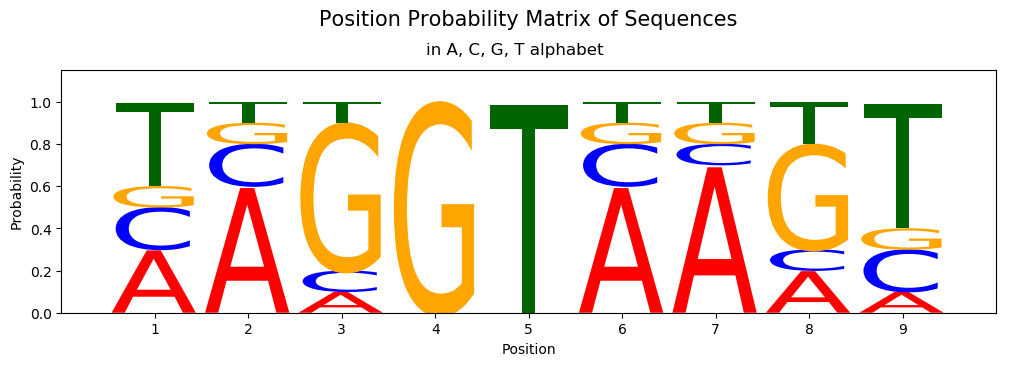
\includegraphics[scale=0.5]{../pss/pss_ppm.png}	
	\end{center}
	\caption{Die Position Probability Matrix (PPM) als Sequenzlogo geplottet. Man sieht den Anteil an C,G,T,A basierend auf der
	Größe des Buchstaben.}
\end{figure}

\bigskip\noindent
Landjaeger ribeye fatback, short ribs pork belly short loin doner. Venison shankle swine pork chop tri-tip. Landjaeger kielbasa ball tip t-bone, shoulder jowl tongue hamburger sausage. Sirloin t-bone cow bacon burgdoggen biltong ribeye filet mignon. Tongue swine cow jerky, venison ground round buffalo chuck bacon turducken leberkas ribeye meatball ham hock strip steak. Ham chicken pig shoulder andouille.

\newgeometry{top=3.04cm, bottom=3.54cm, left=2.04cm, right=2.04cm}
\captionsetup[lstlisting]{format=hang, margin=5pt}
\lstset{
	basicstyle=\color{Black}\ttfamily\normalsize,
	stringstyle=\color{Black}\ttfamily,
	numbers=none,
	captionpos=b,
	breaklines=true
}
\begin{lstlisting}[caption=Der Konsolenoutput des PSS Programms. Als Zielsequenzen zum Berechnen eines Scores wurde dasselbe File verwendet\, wie zum Einlesen des alignierten Sequenzen.]
====================================================================
Position Specific Scoring (PSS)
	by Alen Kocaj

[i] reading source alignments out of 'testing/source'
[i] reading target sequences out of 'testing/target'
====================================================================
[PPM] Position Probability Matrix
	 0    1    2             3             4    5    6    7    8
A  0.3  0.6  0.1  1.000000e-10  1.000000e-10  0.6  0.7  0.2  0.1
C  0.2  0.2  0.1  1.000000e-10  1.000000e-10  0.2  0.1  0.1  0.2
G  0.1  0.1  0.7  1.000000e+00  1.000000e-10  0.1  0.1  0.5  0.1
T  0.4  0.1  0.1  1.000000e-10  1.000000e+00  0.1  0.1  0.2  0.6

[i] plot sequence logo of PPM
[i] figure saved at 'pss_ppm.png'
====================================================================
[PPM] Probability Weight Matrix
		  0         1         2          3          4         5         6  \
A -1.203973 -0.510826 -2.302585 -23.025851 -23.025851 -0.510826 -0.356675   
C -1.609438 -1.609438 -2.302585 -23.025851 -23.025851 -1.609438 -2.302585   
G -2.302585 -2.302585 -0.356675   0.000000 -23.025851 -2.302585 -2.302585   
T -0.916291 -2.302585 -2.302585 -23.025851   0.000000 -2.302585 -2.302585   

		  7         8  
A -1.609438 -2.302585  
C -2.302585 -1.609438  
G -0.693147 -2.302585  
T -1.609438 -0.510826  
====================================================================
[i] scoring targets

# [0th target] #####
> Sequence: GAGGTAAAC
> Log Score by PSS: -7.25646205327

# [1th target] #####
> Sequence: TCCGTAAGT
> Log Score by PSS: -6.89978710933

# [2th target] #####
> Sequence: CAGGTTGGA
> Log Score by PSS: -10.0778409397

# [3th target] #####
> Sequence: ACAGTCAGT
> Log Score by PSS: -8.28608147045

# [4th target] #####
> Sequence: TAGGTCATT
> Log Score by PSS: -5.87016769215

# [5th target] #####
> Sequence: TAGGTACTG
> Log Score by PSS: -8.50922502177

# [6th target] #####
> Sequence: ATGGTAACT
> Log Score by PSS: -7.54414412572

# [7th target] #####
> Sequence: CAGGTATAC
> Log Score by PSS: -8.50922502177

# [8th target] #####
> Sequence: TGTGTGAGT
> Log Score by PSS: -9.38469375912

# [9th target] #####
> Sequence: AAGGTAAGT
> Log Score by PSS: -4.14294674406

====================================================================
[i] thank you and goodnight
=
\end{lstlisting}

\pagebreak
\newgeometry{top=3.04cm, bottom=3.54cm, left=2.04cm, right=2.04cm}
\lstset{
	stringstyle=\color{Red}\ttfamily,
	commentstyle=\color{Green}\ttfamily,
	numbers=left
}
\lstinputlisting[language=Python, caption={main.py}]{../pss/main.py}

\pagebreak
\lstinputlisting[language=Python, caption={pss.py}]{../pss/pss.py}

\pagebreak
\lstinputlisting[language=Python, caption={alphabet.py}]{../pss/alphabet.py}


\end{document}